% SOURCE_AUTHORITY: sga5_fr_workpass.tex, lines 6159--6270 (LF-normalized unit).
% SOURCE_SHA256: 791F4EFFC5E02832D5D77ED03518C8156D6F07E4C8238B03545DB93D883FBB28
\subsection*{6.14}
Sejam $X$ um $G$-$S$-esquema e $j:U\to X$ uma imersão aberta equivariante,
\[
c:C\to X\times_SX
\]
um morfismo de $G$-$S$-esquemas tal que $c_2(=p_2c):C\to X$ seja quase-finito e de dimensão Tor finita. Suponhamos que
\[
c_1^{-1}(U)\subset c_2^{-1}(U).
\]
Têm-se, portanto, quadrados comutativos
\begin{equation}
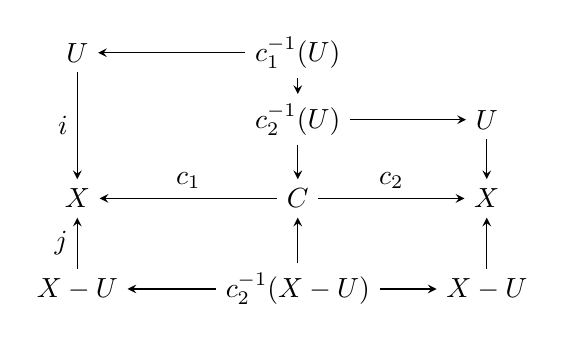
\begin{tikzpicture}[baseline=(current bounding box.center),>=stealth]
\node (U1) at (0,3.0) {$U$};
\node (C1U) at (2.8,3.0) {$c_1^{-1}(U)$};
\node (C2U) at (2.8,2.15) {$c_2^{-1}(U)$};
\node (U2) at (5.2,2.15) {$U$};
\node (X1) at (0,1.15) {$X$};
\node (C) at (2.8,1.15) {$C$};
\node (X2) at (5.2,1.15) {$X$};
\node (XU1) at (0,0) {$X-U$};
\node (C2XU) at (2.8,0) {$c_2^{-1}(X-U)$};
\node (XU2) at (5.2,0) {$X-U$};
\draw[->] (C1U) -- (U1);
\draw[->] (C1U) -- (C2U);
\draw[->] (C2U) -- (U2);
\draw[->] (U1) -- node[left] {$i$} (X1);
\draw[->] (U2) -- (X2);
\draw[->] (C2U) -- (C);
\draw[->] (C2XU) -- (C);
\draw[->] (C) -- node[above] {$c_1$} (X1);
\draw[->] (C) -- node[above] {$c_2$} (X2);
\draw[->] (XU1) -- node[left] {$j$} (X1);
\draw[->] (XU2) -- (X2);
\draw[->] (C2XU) -- (XU1);
\draw[->] (C2XU) -- (XU2);
\end{tikzpicture}
\tag{6.14.1}
\end{equation}
O morfismo de traço
\[
\Tr_{c_2}:c_{2!}\Lambda_C\longrightarrow \Lambda_X
\]
define então uma correspondência $G$-equivariante filtrada
\begin{equation}
\underline c\in\Hom(c_1^*\Lambda_X,c_2^!\Lambda_X),
\tag{6.14.2}
\end{equation}
sendo $\Lambda_X$ dotado da filtração definida pelo submódulo $i_!\Lambda_U$, ou seja,
\[
F^n\Lambda_X=\Lambda_X\quad(n\le0),\qquad
F^1\Lambda_X=i_!\Lambda_U,\qquad
F^n\Lambda_X=0\quad(n\ge1).
\]
O graduado associado é constituído pelas duas correspondências $G$-equivariantes
\[
\operatorname{gr}^0\underline c=\underline c_{X-U,X}
\in\Hom(c_1^*\Lambda_{X-U,X},c_2^!\Lambda_{X-U,X}),
\]
\begin{equation}
\operatorname{gr}^1\underline c=\underline c_{U,X}
\in\Hom(c_1^*\Lambda_{U,X},c_2^!\Lambda_{X-U,X}),
\tag{6.14.3}
\end{equation}
onde pusemos
\[
\Lambda_{X-U,X}=j_*\Lambda_{X-U},\qquad
\Lambda_{U,X}=i_!\Lambda_U.
\]
Tem-se
\begin{equation}
\underline c_{X-U,X}=j_*\underline c_{X-U},
\tag{6.14.4}
\end{equation}
onde
\[
\underline c_{X-U}\in\Hom(c_1^*\Lambda_{X-U},c_2^!\Lambda_{X-U})
\]
é a correspondência definida por $\Tr_{c_2,X-U}$. Escreveremos $\underline c$, $\underline c_{U,X}$, etc., quando quisermos precisar o anel de base.

Esqueçamos a ação de $G$. Têm-se termos locais
\begin{equation}
\Tr_{\Lambda}(\underline c),\quad
\Tr_{\Lambda}(\underline c_{U,X}),\quad
\Tr_{\Lambda}(\underline c_{X-U,X})
\in H^0(X^c,K_{X^c}),
\tag{6.14.5}
\end{equation}
que, em virtude da aditividade dos traços (III 4.13.1), satisfazem a relação
\begin{equation}
\Tr_{\Lambda}(\underline c)
=
\Tr_{\Lambda}(\underline c_{U,X})
+
\Tr_{\Lambda}(\underline c_{X-U,X}).
\tag{6.14.6}
\end{equation}
Além disso, de acordo com 6.14.4, tem-se
\begin{equation}
\Tr_{\Lambda}(\underline c_{X-U,X})
=
j_*^c\Tr_{\Lambda}(\underline c_{X-U}),
\tag{6.14.7}
\end{equation}
onde
\[
j_*^c:H^0((X-U)^c,K_{(X-U)^c})\longrightarrow H^0(X^c,K_{X^c})
\]
é o morfismo de imagem direta definido por $j^c:(X-U)^c\to X^c$. Recordemos (III 4.3) que, se $X$ é suave, $c$ uma imersão fechada e $X^c$ é finito, $\Tr_{\Lambda}(\underline c)$ é a imagem em $\Lambda$ da multiplicidade de interseção $(C\cdot X)$ de $C$ com a diagonal; se, além disso, $X-U$ é suave, $\Tr_{\Lambda}(\underline c_{X-U})$ é a imagem em $\Lambda$ de $(c_2^{-1}(X-U)\cdot(X-U))$. Observemos também que, se $X-U$ é próprio sobre $S$ e $c|X-U$ é a diagonal, então a fórmula de Lefschetz (III 4.7) implica que
\[
\int_{X-U}\Tr(\underline c_{X-U})\in\Lambda
\]
é a característica de Euler--Poincaré de $X-U$ com valores em $\Lambda$.
